
\documentclass[a4paper, 12pt]{article}

% Кодировки
\usepackage[utf8]{inputenc}
\usepackage[T2A]{fontenc}
\usepackage[english,russian]{babel}

% Графика и геометрия
\usepackage{graphicx}
\usepackage{import}
\usepackage{subcaption}
\usepackage{float}
\usepackage{geometry}
\geometry{left=2cm, right=2cm, bottom=2cm, top=2cm}

% Математика
\usepackage{amsmath}
\usepackage{amsfonts}
\usepackage{amstext}

% Таблицы
\usepackage{booktabs}

% Цвета и ссылки
\usepackage[dvipsnames]{xcolor}
\usepackage[colorlinks]{hyperref}
\hypersetup{linkcolor=blue,filecolor=magenta,urlcolor=cyan}

% Прочее
\usepackage{indentfirst}
\usepackage{listings}
\usepackage{src/title} % Убедитесь, что этот файл существует

% Настройки листинга (упрощенные)
\definecolor{intj-bg}{HTML}{2B2B2B}
\definecolor{intj-key}{HTML}{CC7832}
\definecolor{intj-str}{HTML}{6A8759}
\definecolor{intj-comm}{HTML}{808080}
\definecolor{intj-id}{HTML}{A9B7C6}
\definecolor{intj-num}{HTML}{6897BB}


\lstdefinestyle{intellij}{
    language=Python,
    backgroundcolor=\color{intj-bg},
    basicstyle=\ttfamily\small\color{intj-id},
    keywordstyle=\color{intj-key}\bfseries,
    stringstyle=\color{intj-str},
    commentstyle=\itshape\color{intj-comm},
    numberstyle=\color{intj-comm}\tiny,
    stepnumber=1,
    frame=single,
    rulecolor=\color{intj-comm},
    showstringspaces=false,
    breaklines=true,
    tabsize=4,
    extendedchars=true,
}
\lstdefinestyle{intellij2}{
    language=Matlab,
    backgroundcolor=\color{intj-bg},
    basicstyle=\ttfamily\small\color{intj-id},
    keywordstyle=\color{intj-key}\bfseries,
    stringstyle=\color{intj-str},
    commentstyle=\itshape\color{intj-comm},
    numberstyle=\color{intj-comm}\tiny,
    stepnumber=1,
    frame=single,
    rulecolor=\color{intj-comm},
    showstringspaces=false,
    breaklines=true,
    tabsize=4,
    extendedchars=true,
}

%%%%%%%%%%%%%%%%%%%%%%%%%%%%%%%%%%%%%%%%%%%%%%%%
%% Заполнение титульного листа
%%%%%%%%%%%%%%%%%%%%%%%%%%%%%%%%%%%%%%%%%%%%%%%%
\title{
    Лабораторная №1\\
    Построение математической модели двигателя EV3
}

\author{Ануфриев А. С.\\Ндава Маргарет Чити\\Глаголев М.К.}
\affil{
    465029, \href{https://t.me/me_and_no_oneelse}{@me\_and\_no\_oneelse}\\
    505413, \href{https://t.me/margaritaanybody}{@margaritaanybody}\\
    504722, \href{https://t.me/R07331821}{@R07331821}}
\supervisor{\href{https://my.itmo.ru/persons/192059}{Овчаров Алексей Олегович}
}
\abstract{
    В данной работе проведено\\
    экспериментальное исследование динамики двигателя Lego EV3. Построена математическая модель двигателя в виде апериодического звена первого порядка. Определены \\
    статический коэффициент передачи и постоянная времени. Проведено сравнение
    экспериментальных данных с\\ результатами моделирования в Simulink.
}
\keywords{
    ДПТ; Идентификация; Python; MATLAB; Simulink
}

\date{25.03.2026}

%%%%%%%%%%%%%%%%%%%%%%%%%%%%%%%%%%%%%%%%%%%%%%%%
% Начала всего-всего текста. Здесь идет сам документ, все пишется именно сюда
%%%%%%%%%%%%%%%%%%%%%%%%%%%%%%%%%%%%%%%%%%%%%%%%
\begin{document}


    \newpage
    \maketitle
    \newpage
    \tableofcontents
    \newpage


    \section{Постановка задачи}

    \subsection{Цель и задачи исследования}
    Исследуется динамика двигателя EV3. Задачи:
    \begin{enumerate}
        \item Снять переходные процессы при $\pm 20\%, \pm 40\%, \pm 60\%, \pm 80\%, \pm 100\%$.
        \item Определить $k$ и $T_m$ модели.
        \item Построить модель в Simulink.
        \item Сравнить эксперимент, аппроксимацию и Simulink.
        \item Выявить нелинейности.
    \end{enumerate}

    \subsection{Объект исследования}
    Объектом исследования является электродвигатель постоянного тока (ДПТ) с постоянными магнитами, используемый в образовательном конструкторе Lego Mindstorms EV3 (Large Motor). Физическая схема взаимодействия основных элементов двигателя показана на рис.~\ref{fig:motor_scheme}. Ротор (якорь) состоит из обмоток и сердечника. Статор представляет собой неподвижный постоянный магнит. При подаче напряжения \(U\) на обмотки ротора возникает ток \(I\), который, взаимодействуя с полем статора, создает электромагнитный момент \(M_{el}\), приводящий ротор во вращение с угловой скоростью \(\omega\). В процессе вращения в обмотках наводится противо-ЭДС \(\varepsilon_i\), которая препятствует изменению тока.

    \begin{figure}[H]
        \centering
        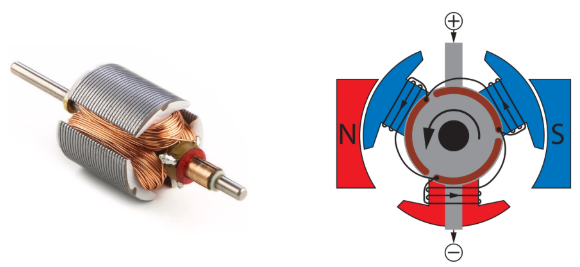
\includegraphics[width=0.8\textwidth]{img.png}
        \caption{Физическая схема двигателя постоянного тока.}
        \label{fig:motor_scheme}
    \end{figure}

    \subsection{Математическая модель двигателя}
    Для описания динамики двигателя используется классическая модель, представленная в теоретической части. Исследуемый двигатель в первом приближении можно рассматривать как апериодическое звено первого порядка:
    \begin{equation}
        W(s) = \frac{k}{T_m s + 1} \Leftrightarrow T_m \frac{d\omega(t)}{dt} + \omega(t) = k \cdot u(t)
        \label{eq:transfer_function}
    \end{equation}
    где \(k\) — коэффициент передачи (рад/(с·\%)), \(T_m\) — электромеханическая постоянная времени (с), \(\omega(t)\) — угловая скорость (рад/с), \(u(t)\) — управляющее напряжение в процентах от максимального.

    При ступенчатом входе \(u(t) = U_0 \cdot \mathbf{1}(t)\):
    \begin{equation}
        \omega(t) = k \cdot U_0 (1 - e^{-t/T_m}), \quad \theta(t) = \int_0^t \omega(\tau) d\tau = k U_0 \left( t - T_m (1 - e^{-t/T_m}) \right)
        \label{eq:step_response}
    \end{equation}
    \newpage


    \section{Экспериментальная установка и методика}

    \subsection{Схема экспериментальной установки}
    Экспериментальная установка (рис.~\ref{fig:exp_setup}) состоит из контроллера EV3, к порту B которого подключен исследуемый двигатель Large Motor. Управление осуществляется с персонального компьютера.

    \begin{figure}[H]
        \centering
        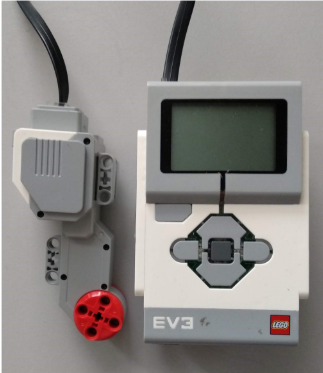
\includegraphics[width=0.8\textwidth]{img_1.png}
        \caption{Общий вид экспериментальной установки.}
        \label{fig:exp_setup}
    \end{figure}

    \subsection{Описание оборудования}
    Использовались: контроллер EV3, двигатель Large Motor, ПК для управления.

    \subsection{Подключение и управление}
    Контроллер подключался по SSH, скрипт передавался через scp, управление — через библиотеку \texttt{ev3dev-lang-python}.

    \subsection{Методика сбора данных}
    Для каждого уровня напряжения ($U \in \{\pm 20\%, \pm 40\%, \pm 60\%, \pm 80\%, \pm 100\%\}$) двигателю подавалось напряжения на 1 сек. Одновременно записывались: время $t$ (мс), угол поворота $\theta(t)$ (град), угловая скорость $\omega(t)$ (град/с). Результаты сохранялись в TXT-файлы.


    \newpage


    \section{Идентификация параметров модели}
    \label{sec:identification}

    \subsection{Методика определения параметров}
    Идентификация параметров модели \(k\) и \(T_m\) производилась по экспериментальным данным угла поворота \(\theta(t)\) с использованием метода наименьших квадратов (МНК) в среде MATLAB. Для аппроксимации использовалась теоретическая зависимость \\\(\hat{\theta}(t) = k U_0 \left( t - T_m (1 - e^{-t/T_m}) \right)\).

    МНК минимизирует сумму квадратов отклонений экспериментальных точек \(\theta_i\) от модельной кривой \(\hat{\theta}(t_i)\):
    \begin{equation}
        S(k, T_m) = \sum_{i=1}^{N} \left( \theta_i - \hat{\theta}(t_i, k, T_m) \right)^2 \rightarrow \min
    \end{equation}

    После нахождения параметров \(k\) и \(T_m\) для каждого уровня напряжения, статический коэффициент передачи \(k\) также был проверен по установившемуся значению скорости \(\omega_{ust}\): \(k = \omega_{ust} / U_0\). Качество аппроксимации оценивалось с помощью коэффициента детерминации \(R^2\), который показывает, какая доля дисперсии экспериментальных данных объясняется моделью:
    \begin{equation}
        R^2 = 1 - \frac{\sum (\theta_i - \hat{\theta}_i)^2}{\sum (\theta_i - \bar{\theta})^2}
    \end{equation}

    \subsection{Результаты}
    На рис.~\ref{fig:params_k}-\ref{fig:params_omega} показаны зависимости параметров модели от управляющего сигнала. Полученные значения сведены в табл.~\ref{tab:parameters_identification}.

    Анализ полученных данных позволяет сделать вывод о нелинейности исследуемого объекта. Видно, что коэффициент передачи \(k\) и постоянная времени \(T_m\) не являются константами, а возрастают с увеличением подаваемого напряжения. Это особенно заметно для \(T_m\), которая при 100\% мощности (0.1046 с) почти в 1.5 раза выше, чем при 20\% (0.0656 с). Такое поведение может объясняться влиянием насыщения магнитной системы, изменением сопротивления обмоток при нагреве или нелинейностью механических характеристик (например, сил трения), которые в упрощенной модели не учитываются.
    \begin{table}[H]
        \centering
        \caption{Параметры передаточной функции двигателя для различных уровней управляющего сигнала}
        \label{tab:parameters_identification}
        \begin{tabular}{|c|c|c|}
            \hline
            \textbf{ШИМ (\%)} & \textbf{$k$ (рад/с/\%)} & \textbf{$T_m$ (с)} \\
            \hline
            $-100$            & 0.1835                  & 0.0912             \\
            $-80$             & 0.1822                  & 0.0935             \\
            $-60$             & 0.1785                  & 0.0759             \\
            $-40$             & 0.1733                  & 0.0708             \\
            $-20$             & 0.1578                  & 0.0634             \\
            \hline
            $+20$             & 0.1652                  & 0.0656             \\
            $+40$             & 0.1829                  & 0.0747             \\
            $+60$             & 0.1889                  & 0.0784             \\
            $+80$             & 0.1928                  & 0.0883             \\
            $+100$            & 0.1967                  & 0.1046             \\
            \hline
            \textbf{Среднее}  & \textbf{0.1802}         & \textbf{0.0806}    \\
            \hline
        \end{tabular}
    \end{table}

    \begin{figure}[H]
        \centering
        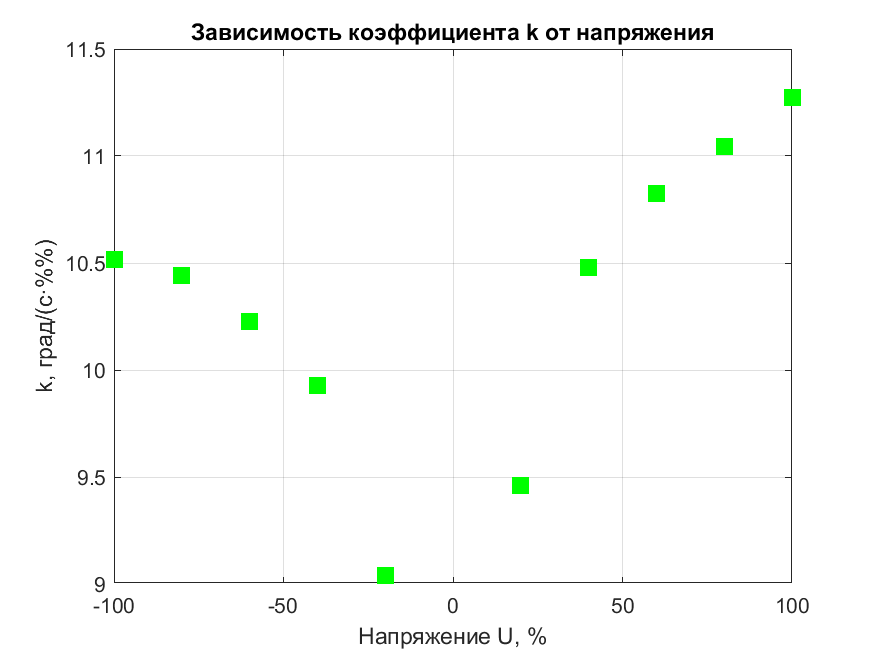
\includegraphics[width=0.9\textwidth]{../matlab/graphs/parameters/k.png}
        \caption{Зависимость коэффициента $k$ от напряжения}
        \label{fig:params_k}
    \end{figure}
    \begin{figure}[H]
        \centering
        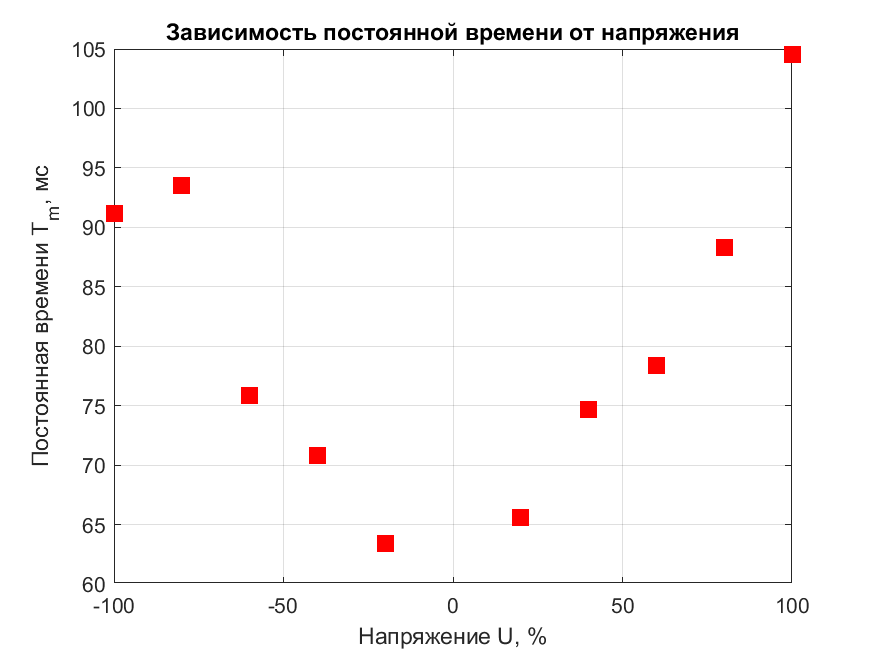
\includegraphics[width=0.9\textwidth]{../matlab/graphs/parameters/Tm.png}
        \caption{Зависимость постоянной времени $T_m$ от напряжения}
        \label{fig:params_Tm}
    \end{figure}
    \begin{figure}[H]
        \centering
        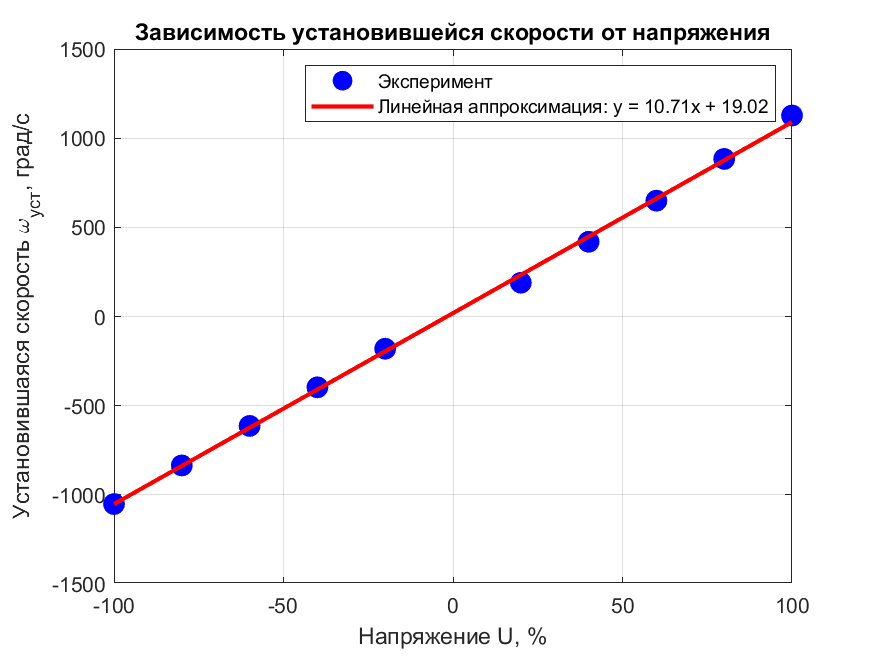
\includegraphics[width=0.9\textwidth]{../matlab/graphs/parameters/omega_steady.png}
        \caption{Установившаяся угловая скорость в зависимости от напряжения}
        \label{fig:params_omega}
    \end{figure}


    \newpage


    \section{Анализ результатов}

    \subsection{Сводные результаты}
    На рис.~\ref{fig:summary_omega} и~\ref{fig:summary_theta} представлены графики для всех пяти положительных и пяти отрицательных напряжений, позволяющие оценить общий характер переходных процессов.

    \begin{figure}[H]
        \centering
        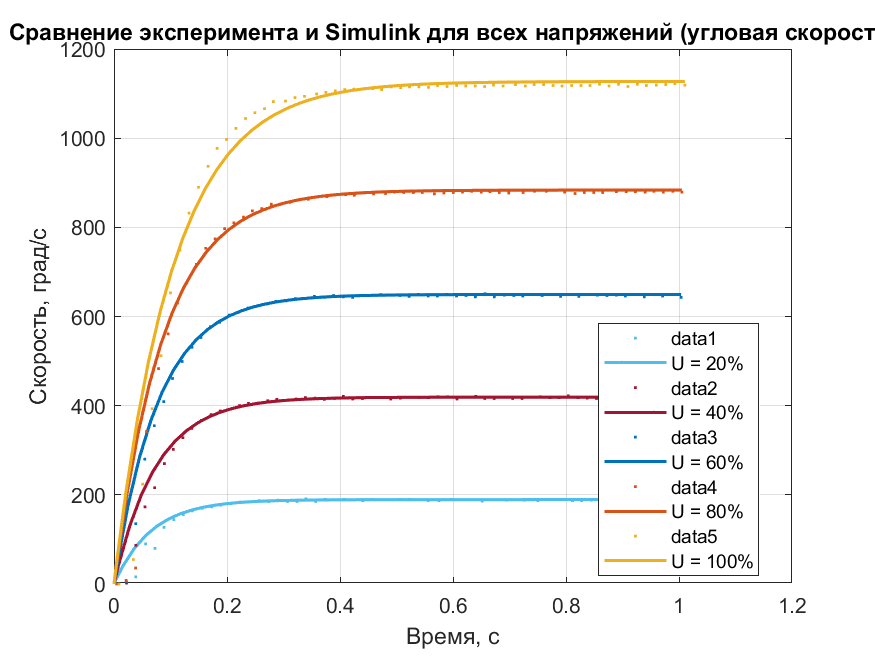
\includegraphics[width=0.95\textwidth]{../matlab/graphs/comparison/all_velocities_comparison.png}
        \caption{Сравнение экспериментальных данных и моделирования в Simulink для угловой скорости при различных уровнях управляющего сигнала.}
        \label{fig:summary_omega}
    \end{figure}

    \begin{figure}[H]
        \centering
        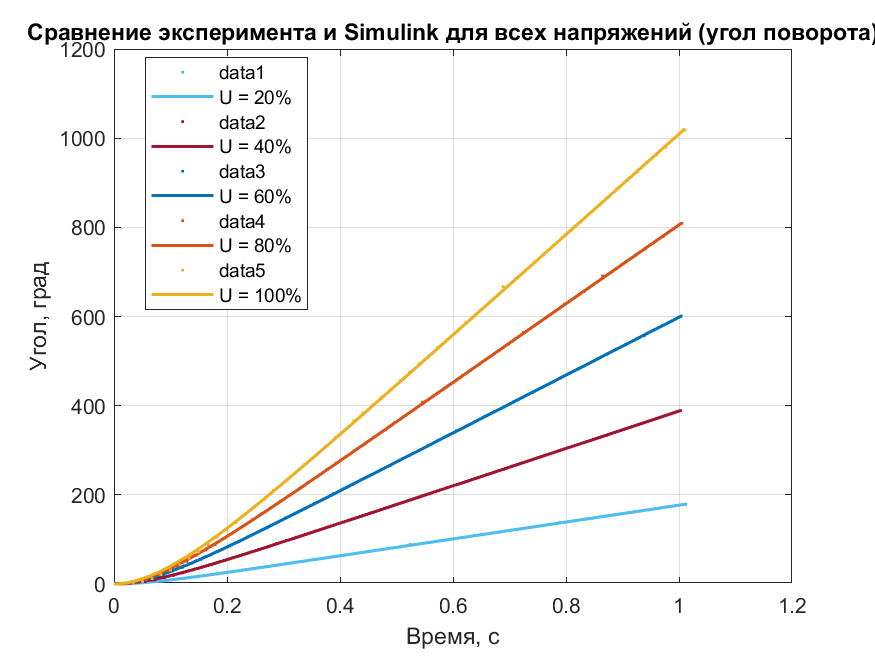
\includegraphics[width=0.95\textwidth]{../matlab/graphs/comparison/all_angles_comparison.png}
        \caption{Сравнение экспериментальных данных и моделирования в Simulink для угла поворота при различных уровнях управляющего сигнала.}
        \label{fig:summary_theta}
    \end{figure}

    \subsection{Сравнение результатов}
    На рис.~\ref{fig:detailed_group1}-\ref{fig:detailed_group4} показаны углы и скорости для всех режимов: синие точки — опыт, красная линия — апроксимация.


    \begin{figure}[H]
        \centering
        \begin{subfigure}[b]{0.48\textwidth}
            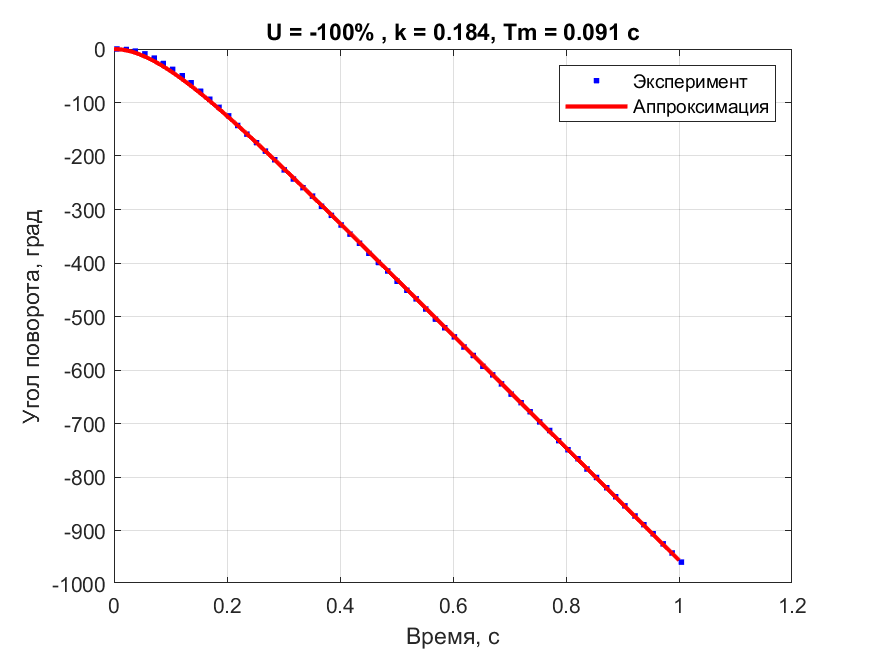
\includegraphics[width=\textwidth]{../matlab/graphs/angles/angle_-100.png}
            \caption{Угол при -100\%}
        \end{subfigure}
        \begin{subfigure}[b]{0.48\textwidth}
            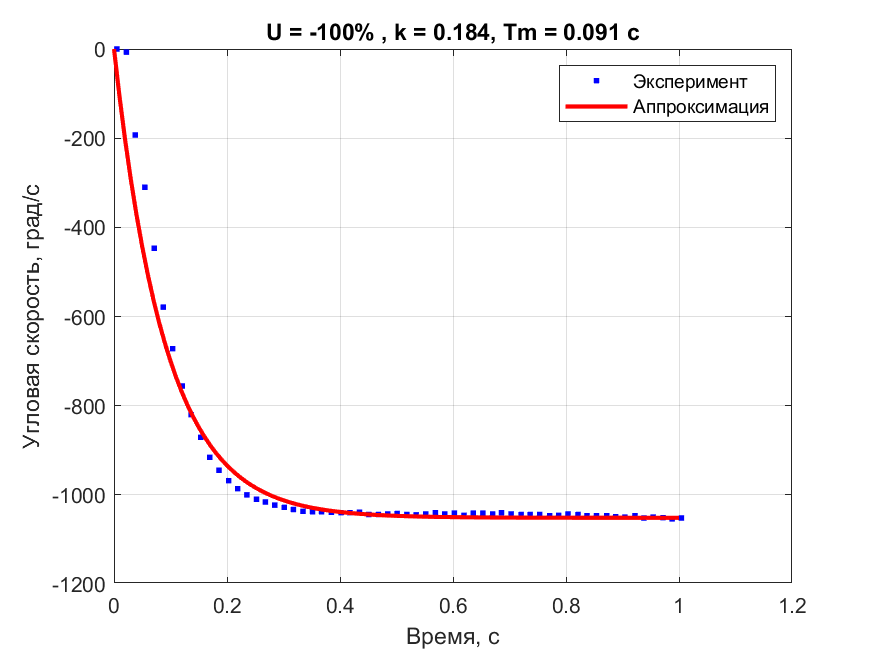
\includegraphics[width=\textwidth]{../matlab/graphs/velocities/velocity_-100.png}
            \caption{Скорость при -100\%}
        \end{subfigure}
        \begin{subfigure}[b]{0.48\textwidth}
            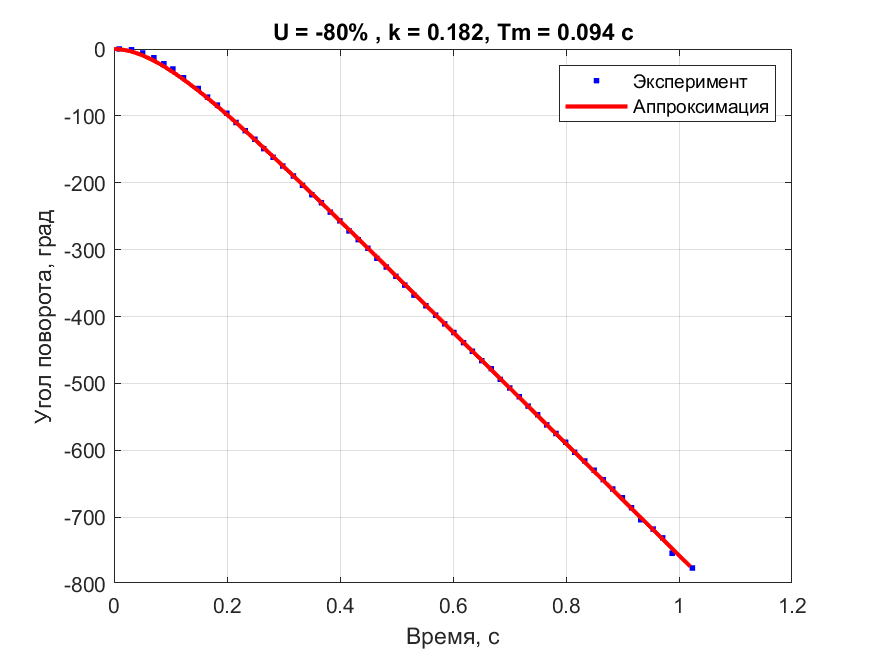
\includegraphics[width=\textwidth]{../matlab/graphs/angles/angle_-80.png}
            \caption{Угол при -80\%}
        \end{subfigure}
        \begin{subfigure}[b]{0.48\textwidth}
            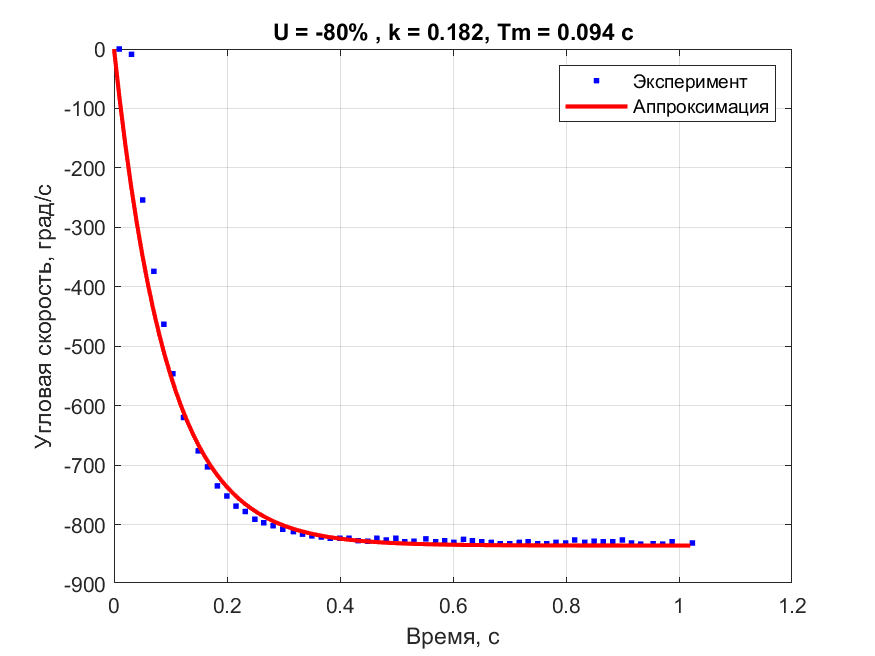
\includegraphics[width=\textwidth]{../matlab/graphs/velocities/velocity_-80.png}
            \caption{Скорость при -80\%}
        \end{subfigure}
        \begin{subfigure}[b]{0.48\textwidth}
            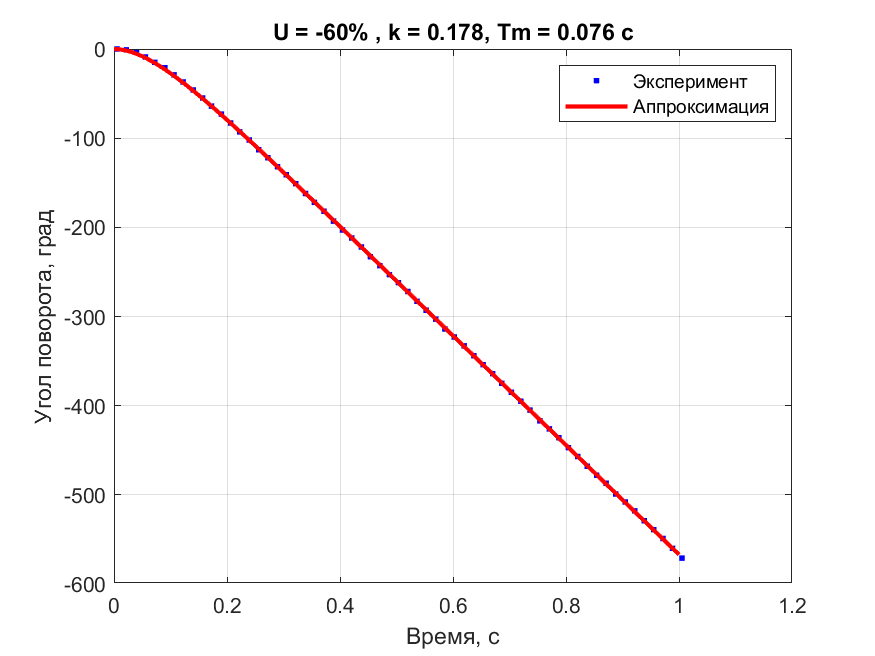
\includegraphics[width=\textwidth]{../matlab/graphs/angles/angle_-60.png}
            \caption{Угол при -60\%}
        \end{subfigure}
        \begin{subfigure}[b]{0.48\textwidth}
            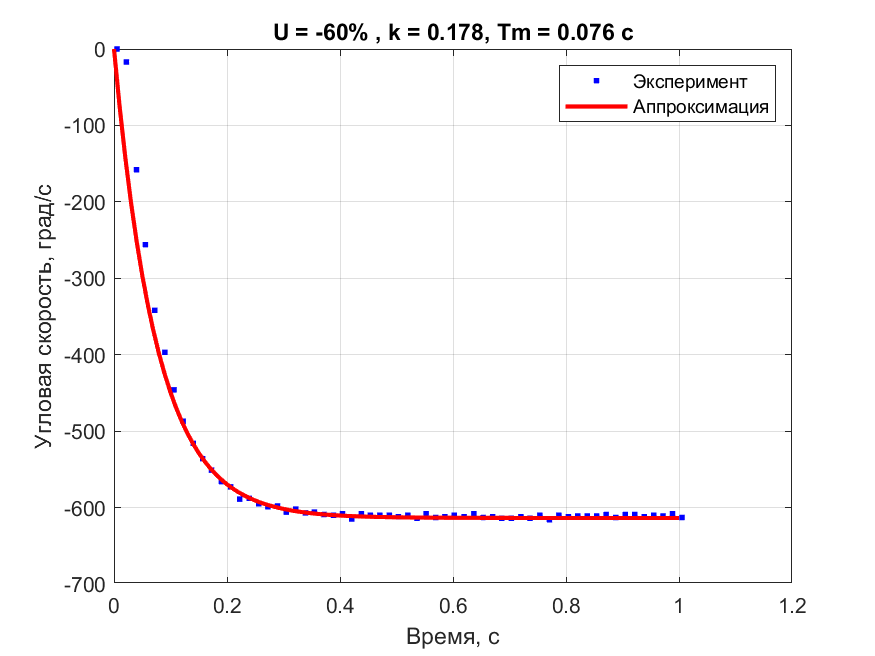
\includegraphics[width=\textwidth]{../matlab/graphs/velocities/velocity_-60.png}
            \caption{Скорость при -60\%}
        \end{subfigure}
        \caption{Для максимальных напряжений график растет быстро, что делает кривизну переходного процесса менее заметной.}


        \label{fig:detailed_group1}
    \end{figure}

    \begin{figure}[H]
        \centering
        \begin{subfigure}[b]{0.48\textwidth}
            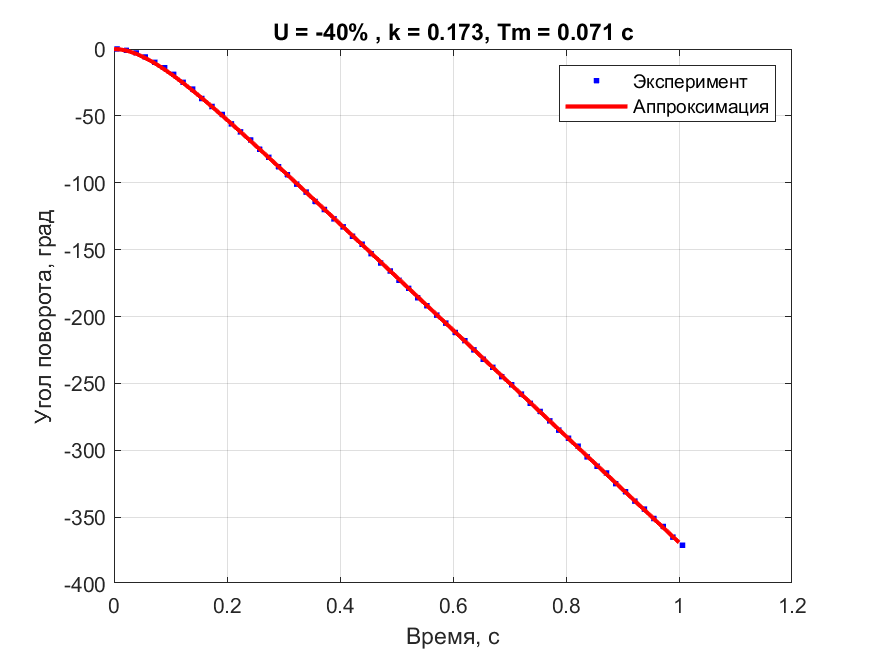
\includegraphics[width=\textwidth]{../matlab/graphs/angles/angle_-40.png}
            \caption{Угол при -40\%}
        \end{subfigure}
        \begin{subfigure}[b]{0.48\textwidth}
            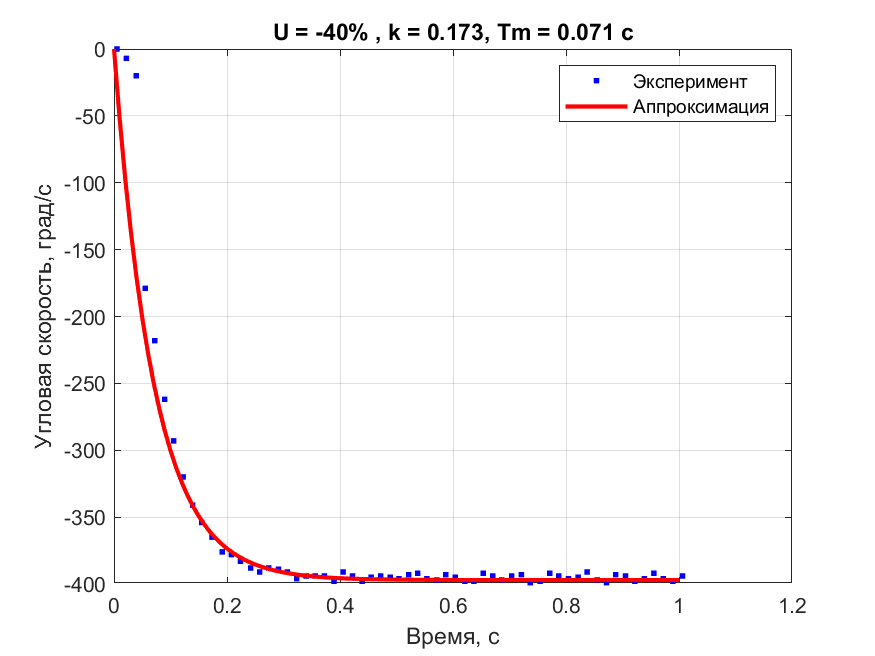
\includegraphics[width=\textwidth]{../matlab/graphs/velocities/velocity_-40.png}
            \caption{Скорость при -40\%}
        \end{subfigure}
        \begin{subfigure}[b]{0.48\textwidth}
            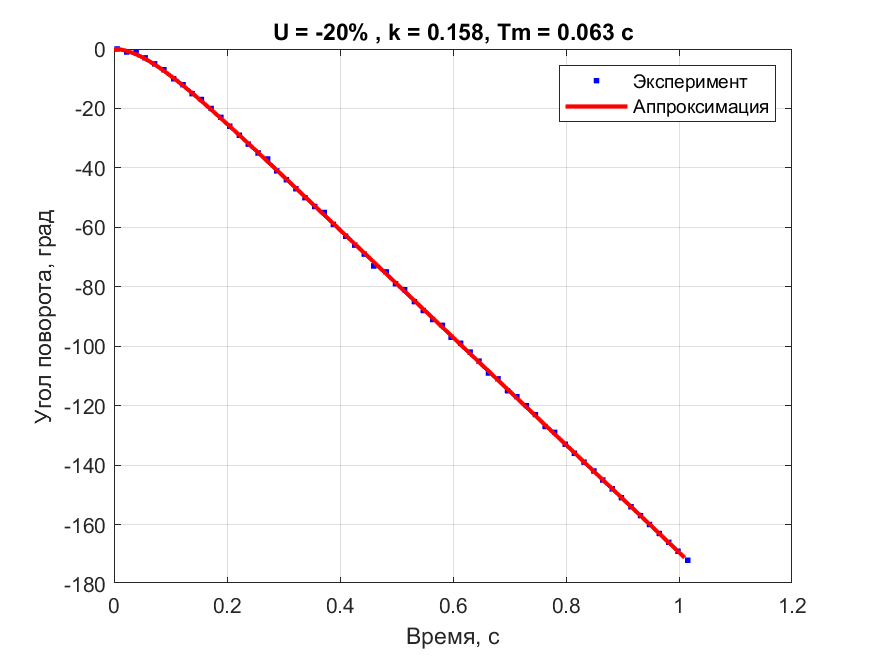
\includegraphics[width=\textwidth]{../matlab/graphs/angles/angle_-20.png}
            \caption{Угол при -20\%}
        \end{subfigure}
        \begin{subfigure}[b]{0.48\textwidth}
            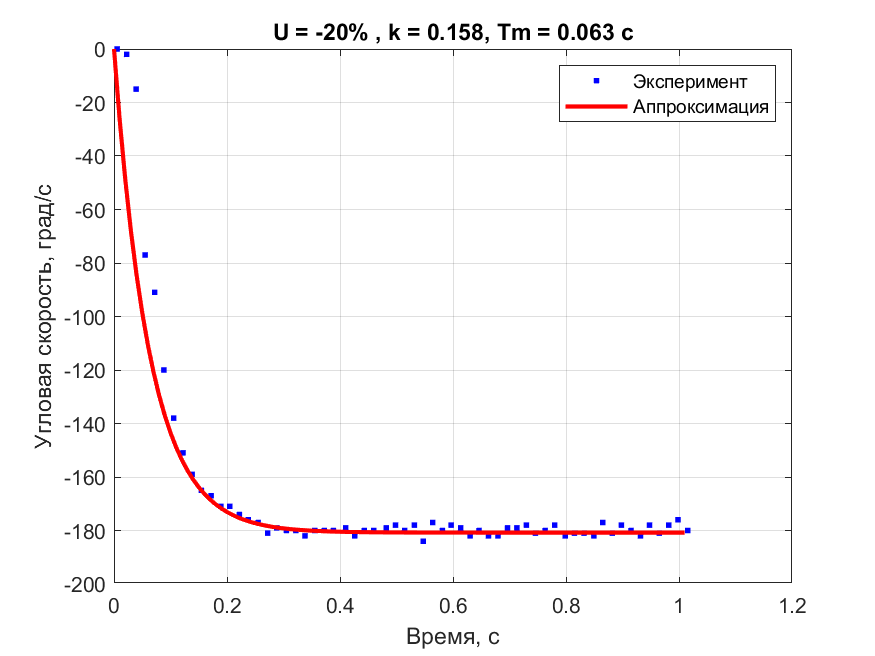
\includegraphics[width=\textwidth]{../matlab/graphs/velocities/velocity_-20.png}
            \caption{Скорость при -20\%}
        \end{subfigure}
                        \caption{Средние значения.Кривизну хорошо видно}

        \label{fig:detailed_group2}
    \end{figure}

    \begin{figure}[H]
        \centering
        \begin{subfigure}[b]{0.48\textwidth}
            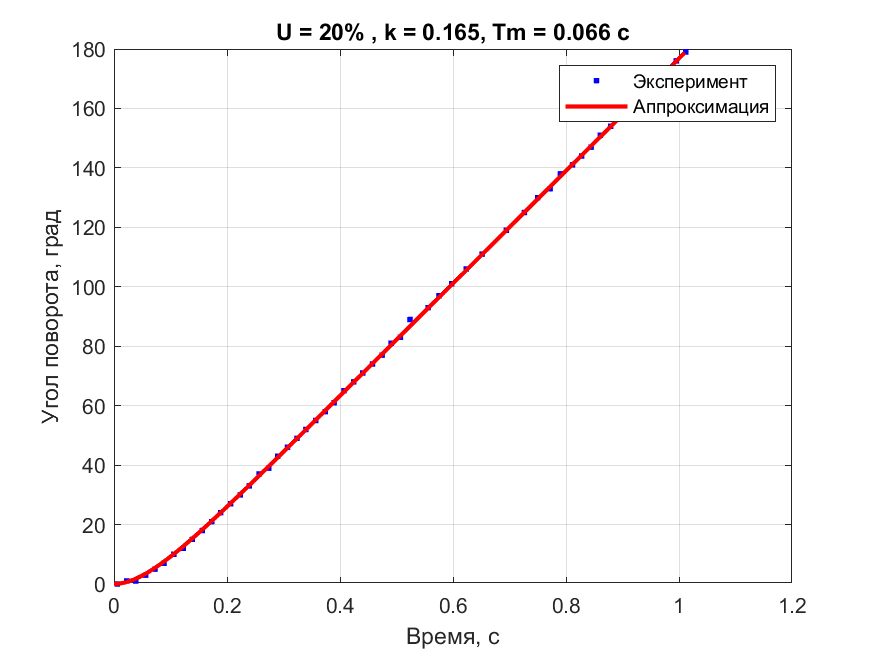
\includegraphics[width=\textwidth]{../matlab/graphs/angles/angle_20.png}
            \caption{Угол при +20\%}
        \end{subfigure}
        \begin{subfigure}[b]{0.48\textwidth}
            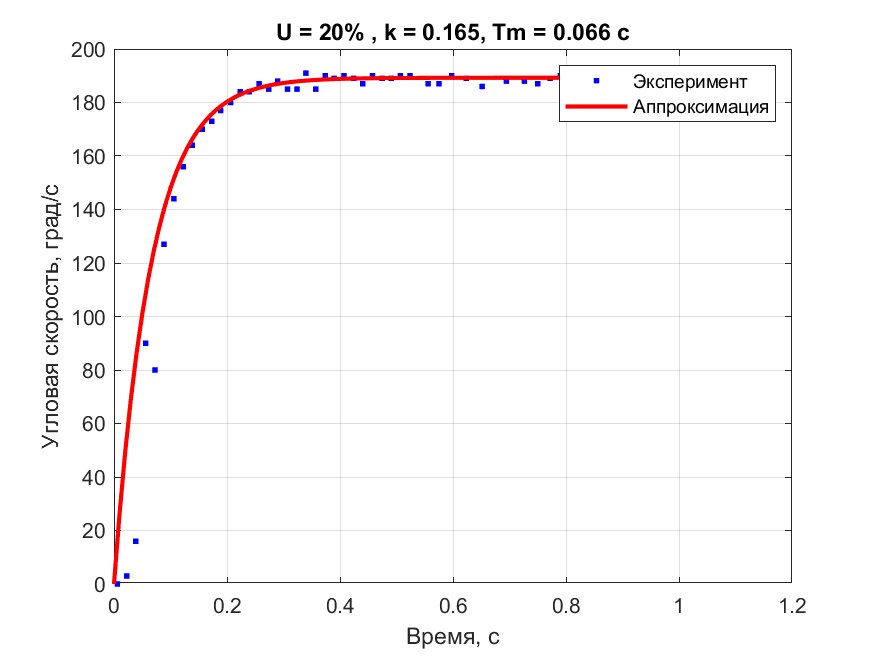
\includegraphics[width=\textwidth]{../matlab/graphs/velocities/velocity_20.png}
            \caption{Скорость при +20\%}
        \end{subfigure}
        \begin{subfigure}[b]{0.48\textwidth}
            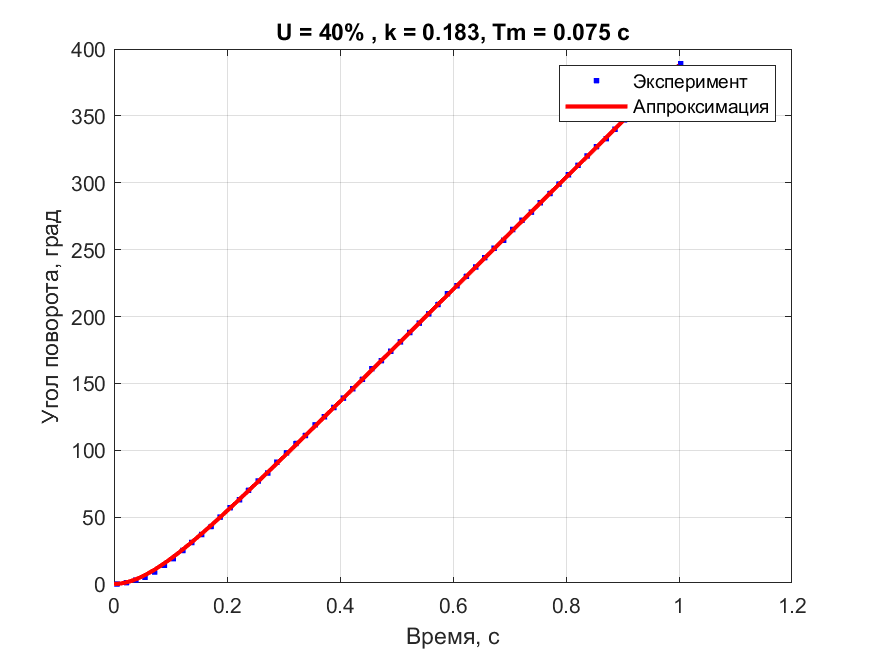
\includegraphics[width=\textwidth]{../matlab/graphs/angles/angle_40.png}
            \caption{Угол при +40\%}
        \end{subfigure}
        \begin{subfigure}[b]{0.48\textwidth}
            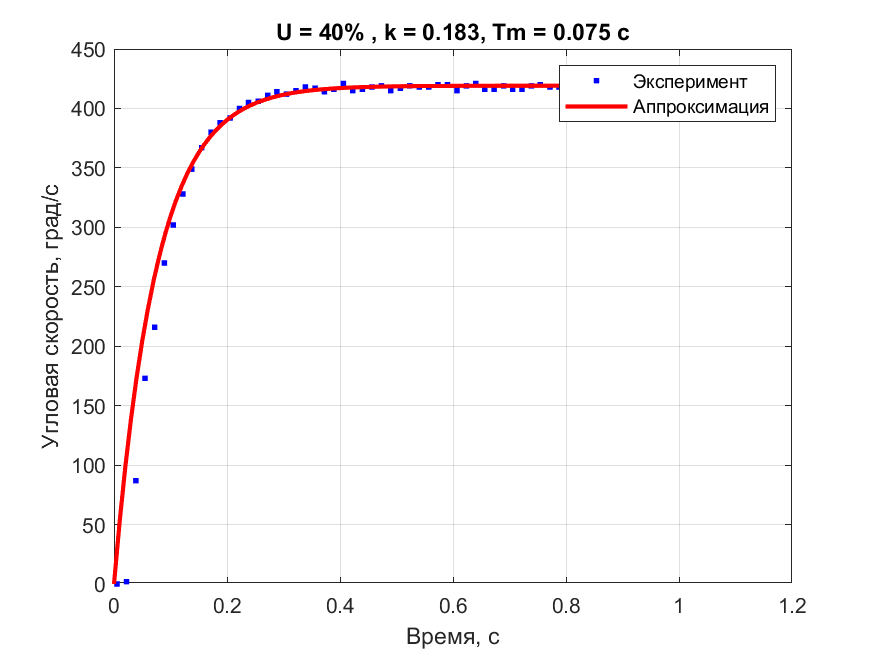
\includegraphics[width=\textwidth]{../matlab/graphs/velocities/velocity_40.png}
            \caption{Скорость при +40\%}
        \end{subfigure}
        \begin{subfigure}[b]{0.48\textwidth}
            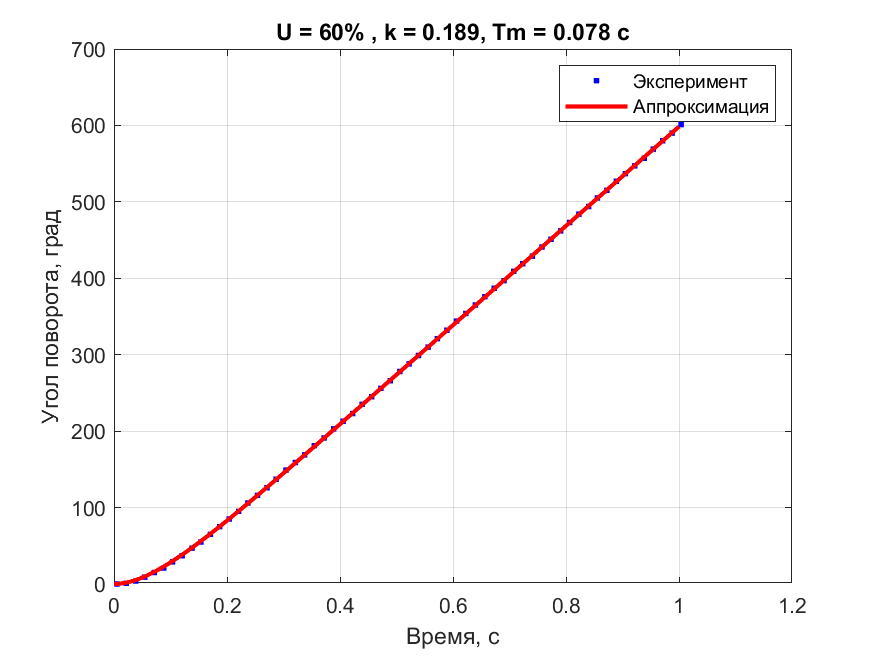
\includegraphics[width=\textwidth]{../matlab/graphs/angles/angle_60.png}
            \caption{Угол при +60\%}
        \end{subfigure}
        \begin{subfigure}[b]{0.48\textwidth}
            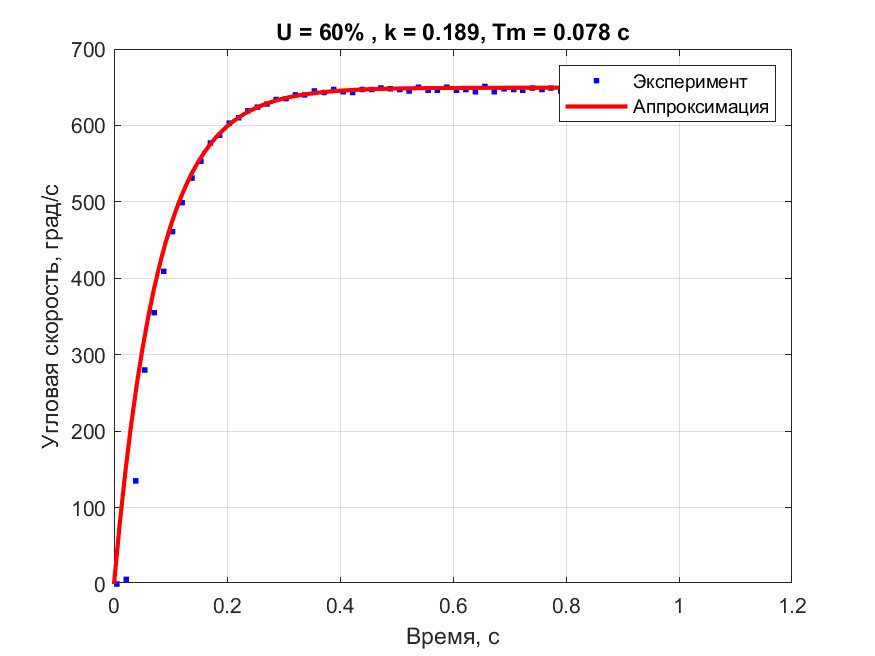
\includegraphics[width=\textwidth]{../matlab/graphs/velocities/velocity_60.png}
            \caption{Скорость при +60\%}
        \end{subfigure}
                \caption{Средние значения.}

        \label{fig:detailed_group3}
    \end{figure}

    \begin{figure}[H]
        \centering
        \begin{subfigure}[b]{0.48\textwidth}
            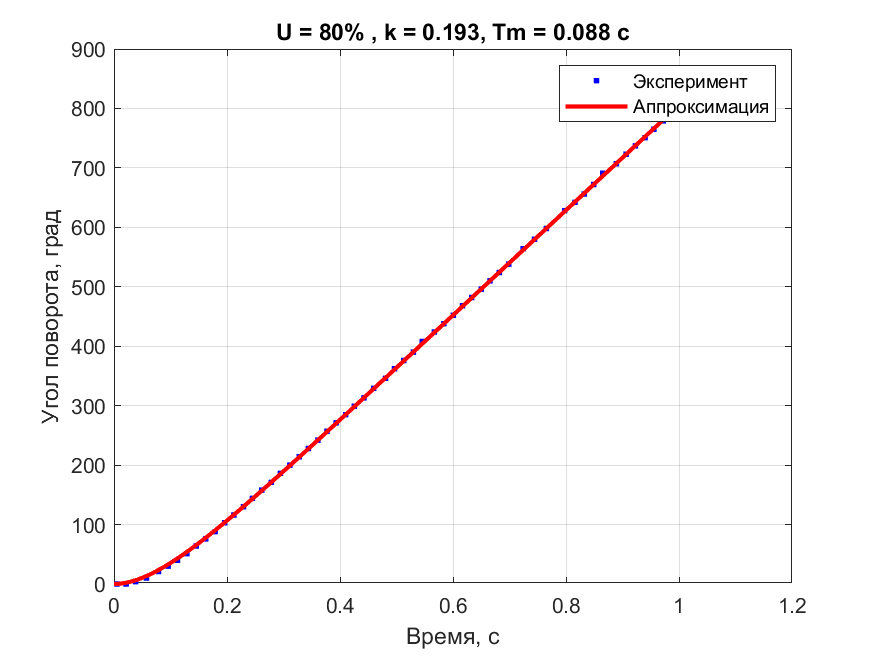
\includegraphics[width=\textwidth]{../matlab/graphs/angles/angle_80.png}
            \caption{Угол при +80\%}
        \end{subfigure}
        \begin{subfigure}[b]{0.48\textwidth}
            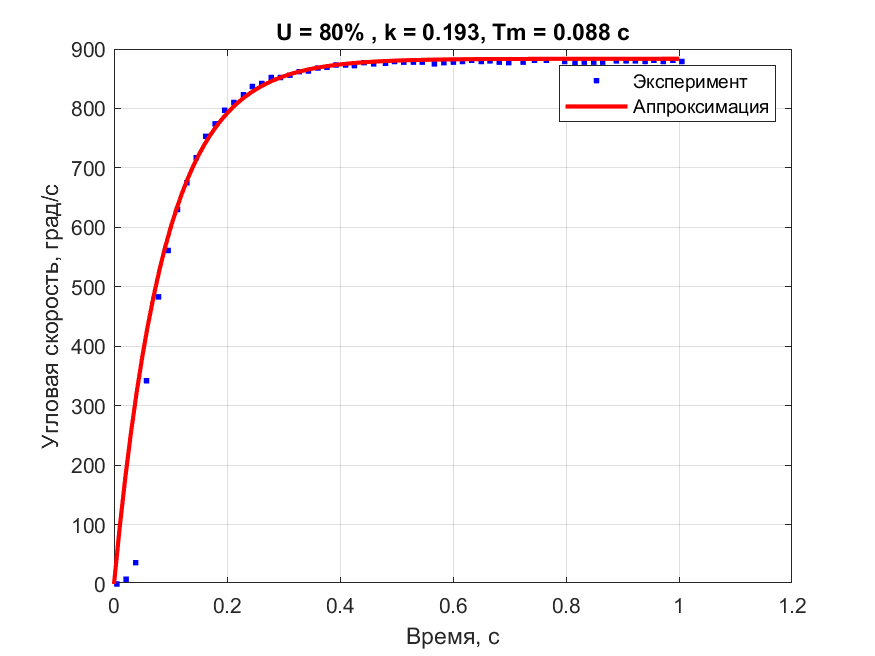
\includegraphics[width=\textwidth]{../matlab/graphs/velocities/velocity_80.png}
            \caption{Скорость при +80\%}
        \end{subfigure}
        \begin{subfigure}[b]{0.48\textwidth}
            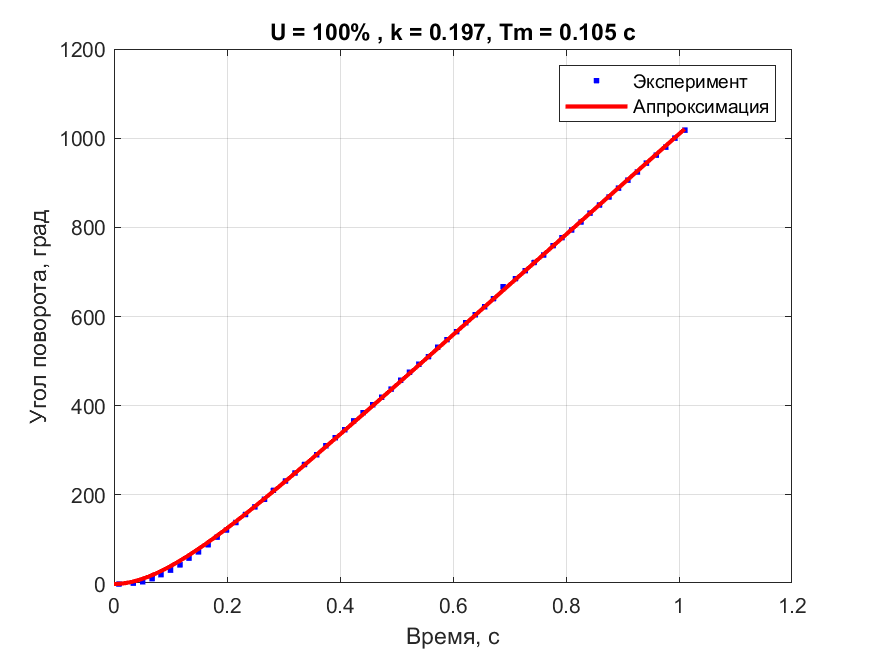
\includegraphics[width=\textwidth]{../matlab/graphs/angles/angle_100.png}
            \caption{Угол при +100\%}
        \end{subfigure}
        \begin{subfigure}[b]{0.48\textwidth}
            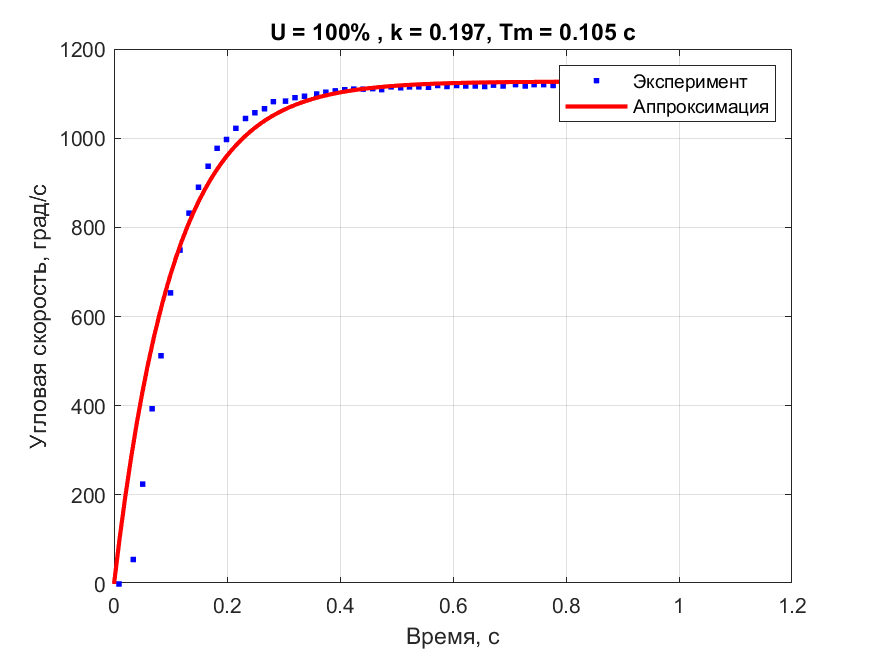
\includegraphics[width=\textwidth]{../matlab/graphs/velocities/velocity_100.png}
            \caption{Скорость при +100\%}
        \end{subfigure}
        \caption{Для максимальных напряжений график растет быстро, что делает кривизну переходного процесса менее заметной.}
        \label{fig:detailed_group4}
    \end{figure}


    \newpage


    \section{Моделирование в Simulink}
    \label{sec:simulation}

    Для верификации полученной математической модели было проведено имитационное моделирование в среде Simulink. Структурная схема модели (рис.~\ref{fig:simulink_scheme}) построена на основе дифференциального уравнения \(T_m \dot{\omega} + \omega = k u(t)\) и позволяет получить зависимости угловой скорости \(\omega(t)\) и угла поворота \(\theta(t)\) от времени.

    \subsection{Описание структурной схемы}
    Схема (рис.~\ref{fig:simulink_scheme}) реализована следующим образом:
    \begin{itemize}
        \item Блок \texttt{Constant} задает значение управляющего сигнала \(U\) (\%).
        \item Блок \texttt{Gain} с коэффициентом \(k\) формирует установившееся значение скорости \(\omega_{ycm} = kU\).
        \item Сумматор \texttt{Sum} вычитает из \(\omega_{ycm}\) текущее значение скорости \(\omega(t)\), поступающее с выхода интегратора, формируя тем самым сигнал ошибки \(\omega_{ycm} - \omega(t)\).
        \item Блок \texttt{Gain1} с коэффициентом \(1/T_m\) масштабирует сигнал ошибки в ускорение \(\dot{\omega}\).
        \item Интегратор \texttt{Integrator1} интегрирует ускорение и возвращает текущее значение скорости \(\omega(t)\), замыкая контур обратной связи.
        \item Второй интегратор \texttt{Integrator} интегрирует скорость и возвращает угол поворота \(\theta(t)\).
        \item Блоки \texttt{To File} служат для сохранения результатов моделирования в файлы \texttt{omega\_data.mat} и \texttt{theta\_data.mat}.
    \end{itemize}

    \begin{figure}[H]
        \centering
        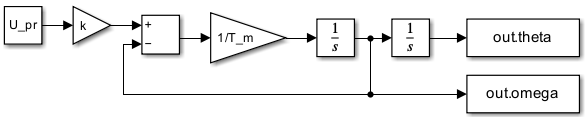
\includegraphics[width=0.9\textwidth]{../matlab/shema.png}
        \caption{Структурная схема модели двигателя EV3 в Simulink.}
        \label{fig:simulink_scheme}
    \end{figure}

    \subsection{Результаты моделирования}
    На рис.~\ref{fig:simulink_comparison1} и \ref{fig:simulink_comparison2} представлено сравнение результатов моделирования в Simulink с экспериментальными данными и аппроксимирующей кривой. Синие точки обозначают экспериментальные данные, красная линия — аппроксимирующую кривую, зеленая линия — результаты моделирования в Simulink.

    \begin{figure}[H]
        \centering
        \begin{subfigure}[b]{0.48\textwidth}
            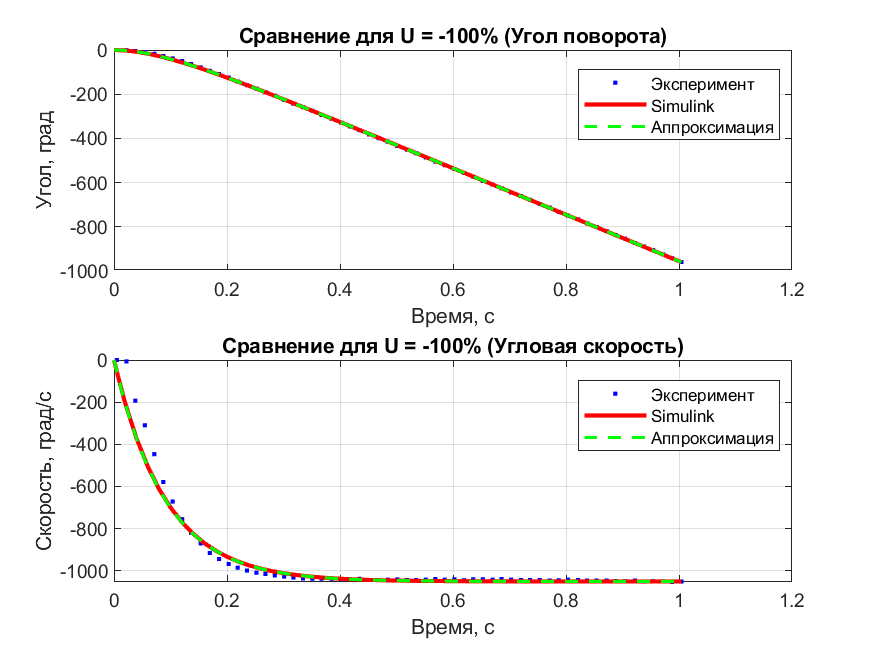
\includegraphics[width=\textwidth]{../matlab/graphs/comparison/comparison_-100.png}
            \caption{Сравнение при -100\%}
        \end{subfigure}
        \begin{subfigure}[b]{0.48\textwidth}
            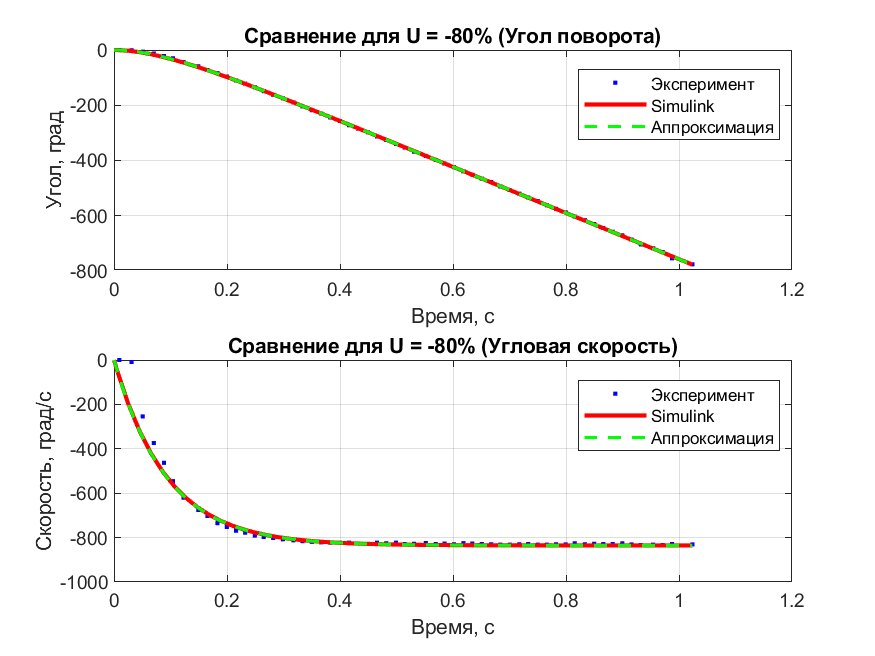
\includegraphics[width=\textwidth]{../matlab/graphs/comparison/comparison_-80.png}
            \caption{Сравнение при -80\%}
        \end{subfigure}
        \begin{subfigure}[b]{0.48\textwidth}
            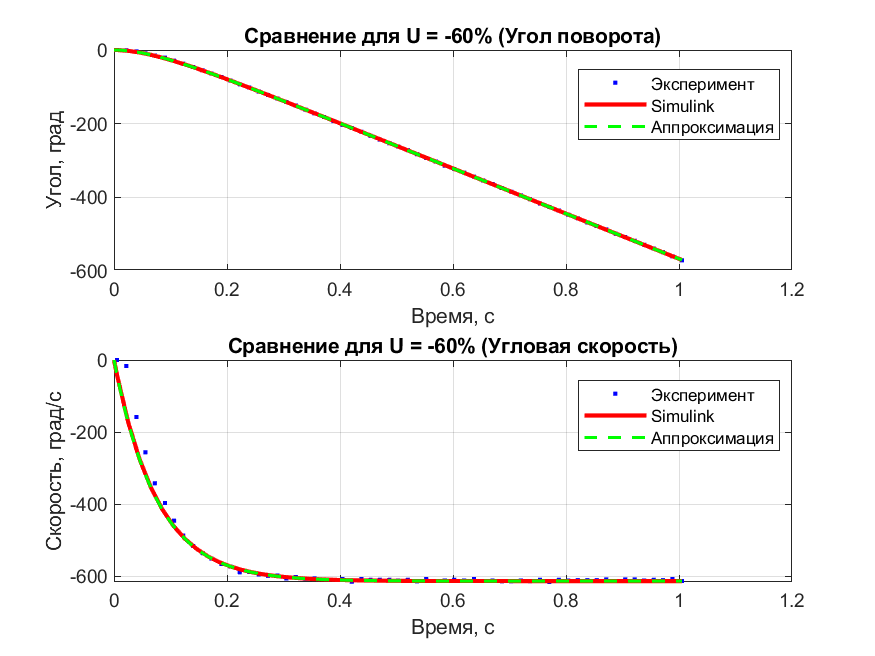
\includegraphics[width=\textwidth]{../matlab/graphs/comparison/comparison_-60.png}
            \caption{Сравнение при -60\%}
        \end{subfigure}
        \begin{subfigure}[b]{0.48\textwidth}
            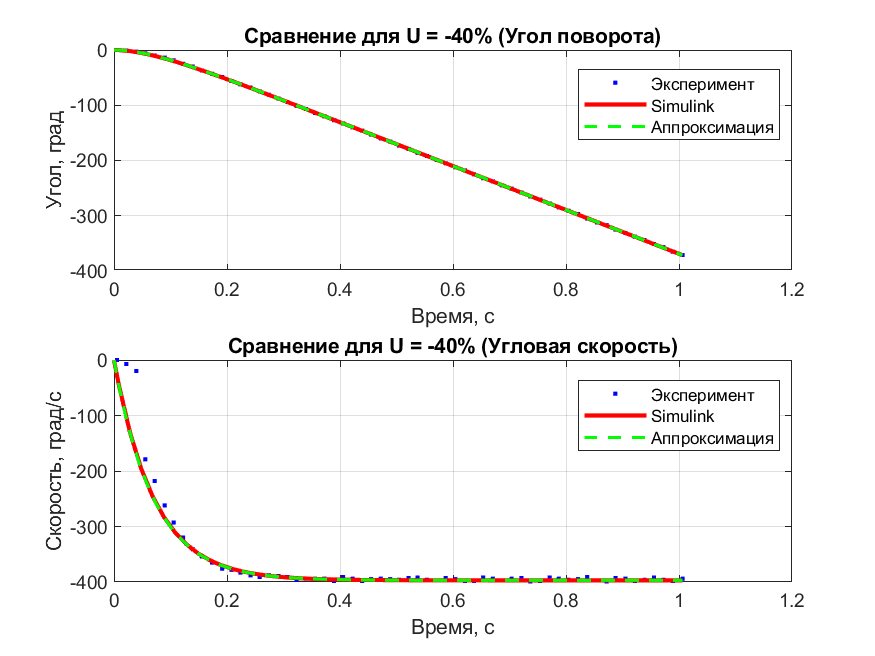
\includegraphics[width=\textwidth]{../matlab/graphs/comparison/comparison_-40.png}
            \caption{Сравнение при -40\%}
        \end{subfigure}
        \begin{subfigure}[b]{0.48\textwidth}
            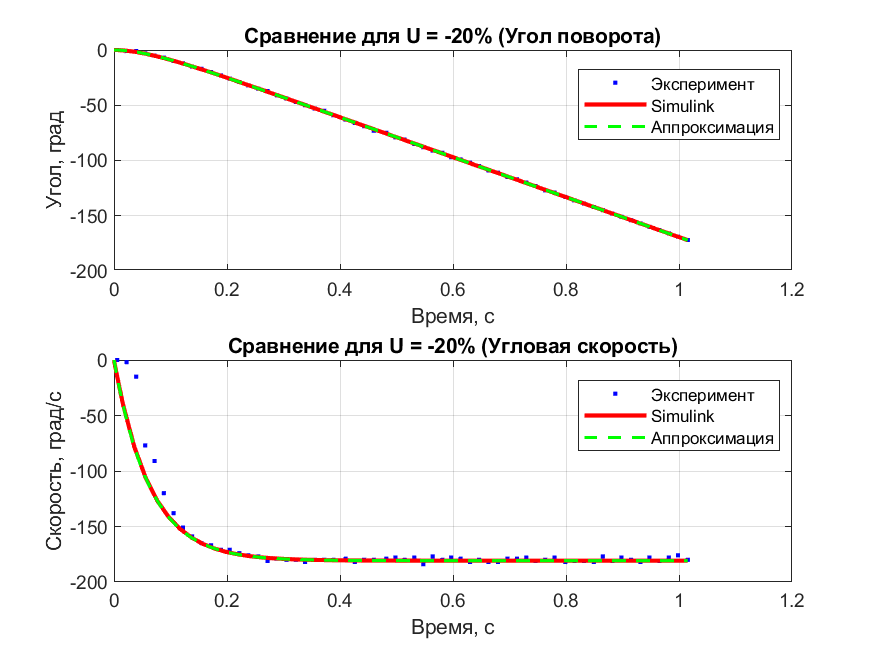
\includegraphics[width=\textwidth]{../matlab/graphs/comparison/comparison_-20.png}
            \caption{Сравнение при -20\%}
        \end{subfigure}
        \caption{Сравнение результатов для отрицательных напряжений. Хорошее совпадение кривых подтверждает адекватность выбранной математической модели.}
        \label{fig:simulink_comparison1}
    \end{figure}

    \begin{figure}[H]
        \centering
        \begin{subfigure}[b]{0.48\textwidth}
            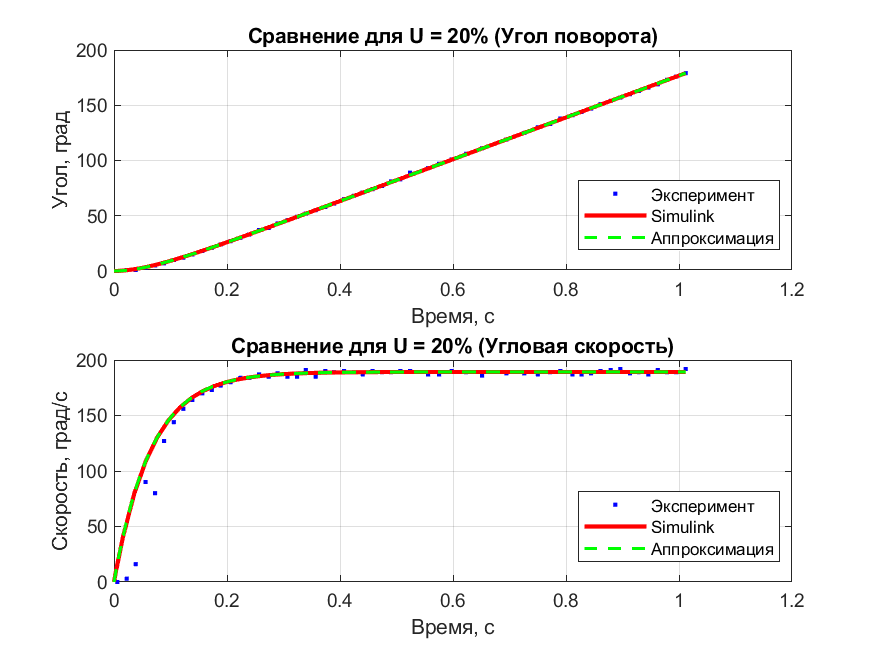
\includegraphics[width=\textwidth]{../matlab/graphs/comparison/comparison_20.png}
            \caption{Сравнение при +20\%}
        \end{subfigure}
        \begin{subfigure}[b]{0.48\textwidth}
            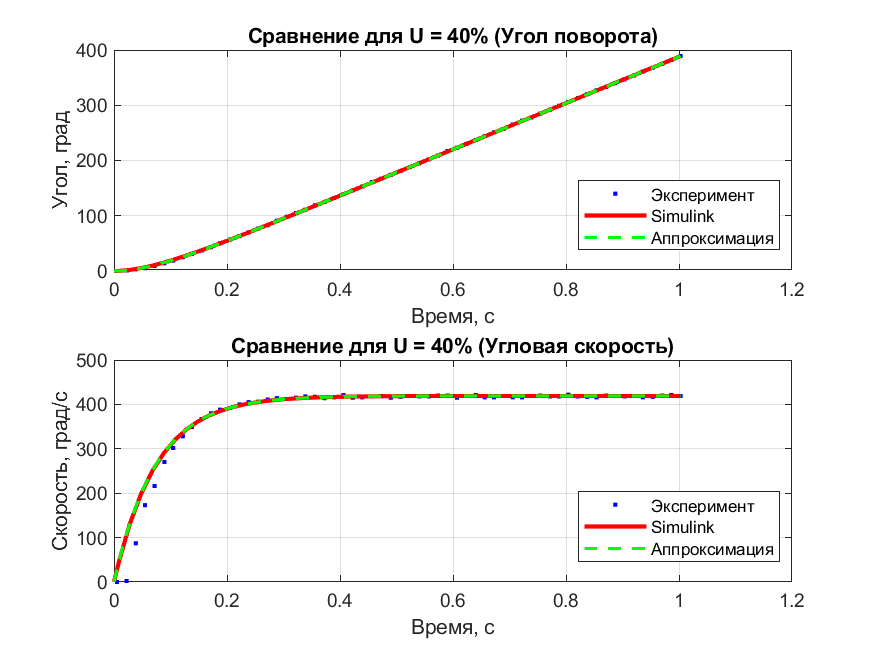
\includegraphics[width=\textwidth]{../matlab/graphs/comparison/comparison_40.png}
            \caption{Сравнение при +40\%}
        \end{subfigure}
        \begin{subfigure}[b]{0.48\textwidth}
            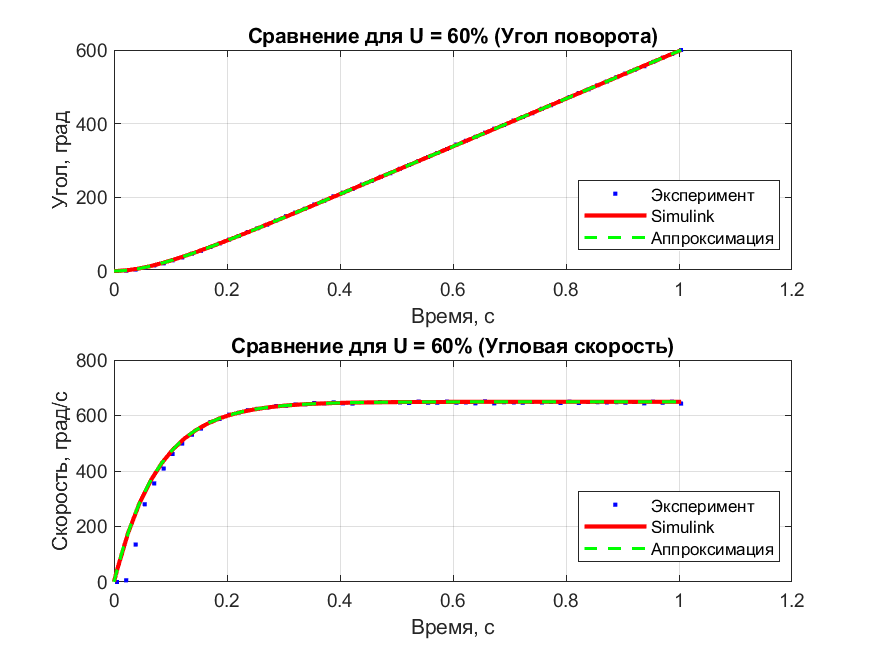
\includegraphics[width=\textwidth]{../matlab/graphs/comparison/comparison_60.png}
            \caption{Сравнение при +60\%}
        \end{subfigure}
        \begin{subfigure}[b]{0.48\textwidth}
            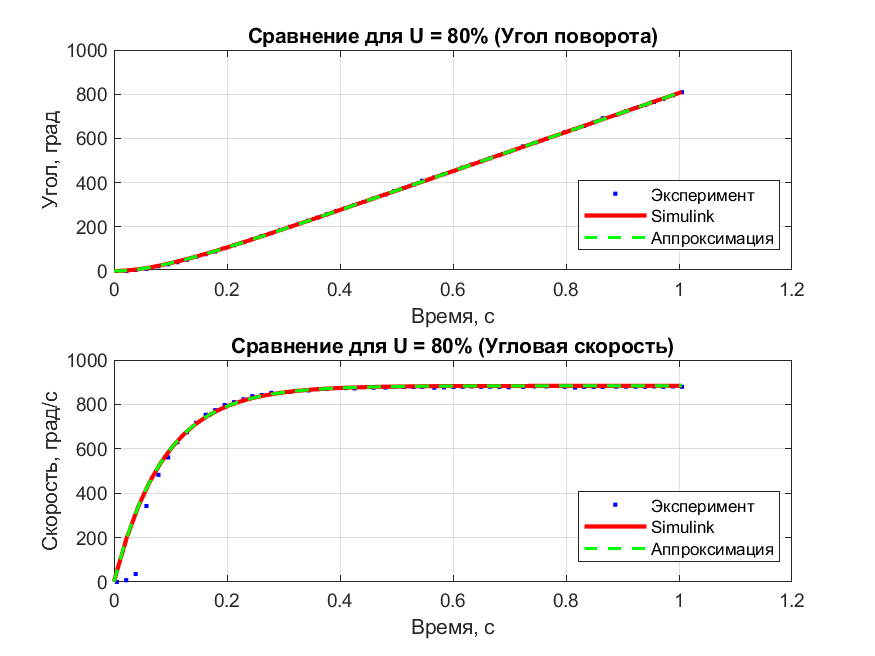
\includegraphics[width=\textwidth]{../matlab/graphs/comparison/comparison_80.png}
            \caption{Сравнение при +80\%}
        \end{subfigure}
        \begin{subfigure}[b]{0.48\textwidth}
            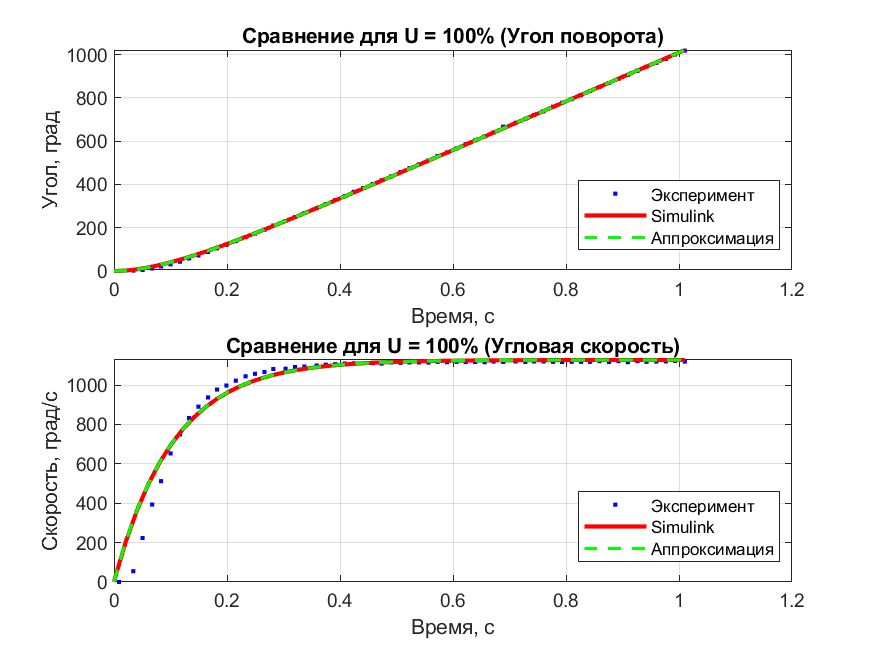
\includegraphics[width=\textwidth]{../matlab/graphs/comparison/comparison_100.png}
            \caption{Сравнение при +100\%}
        \end{subfigure}
        \caption{Сравнение результатов для положительных напряжений. Хорошее совпадение кривых подтверждает адекватность выбранной математической модели.}
        \label{fig:simulink_comparison2}
    \end{figure}
    \newpage


    \section{Выводы}
    В ходе выполнения лабораторной работы все поставленные задачи были успешно решены:
    \begin{enumerate}
        \item Проведены эксперименты по снятию переходных процессов двигателя EV3 для 10 уровней управляющего сигнала в диапазоне от \(-100\%\) до \(+100\%\).
        \item Определены параметры математической модели апериодического звена первого порядка. Для положительных напряжений средний статический коэффициент передачи составил \(k \approx 0.18\) рад/(с·\%), а средняя постоянная времени \(T_m \approx 0.081\) с.
        \item Выявлена нелинейность исследуемого объекта: параметры модели \(k\) и \(T_m\) не являются постоянными и зависят от величины управляющего сигнала. Это указывает на то, что модель первого порядка является лишь приближением, достаточным для многих инженерных задач, но не описывающим поведение системы во всем диапазоне с абсолютной точностью.
        \item Построенная в Simulink модель с использованием средних параметров показала хорошее совпадение с экспериментальными данными, что подтверждает адекватность выбранного подхода для моделирования динамики двигателя EV3.
    \end{enumerate}
    Таким образом, цель работы достигнута: на основе экспериментальных данных построена и верифицирована математическая модель двигателя EV3.

    \newpage


    \section{Программы}

    \subsection{Программа EV3}
    \begin{lstlisting}[style=intellij,basicstyle=\color{intj-id}]
from ev3dev2.motor import LargeMotor, OUTPUT_B
import time

motorA = LargeMotor(OUTPUT_B)
voltages = [100, 80, 60, 40, 20, -20, -40, -60, -80, -100]

try:
    for vol in voltages:
        timeStart = time.time()
        startPos = motorA.position
        name = "data" + str(vol) + ".txt"
        file = open(name, "w")

        while True:
            timeNow = time.time() - timeStart
            motorA.run_direct(duty_cycle_sp=vol)
            pos = motorA.position - startPos
            file.write(str(timeNow) + " " + str(pos) + " " + str(motorA.speed) + "\n")

            if timeNow > 1:
                motorA.run_direct(duty_cycle_sp=0)
                break

            time.sleep(0.01)


        file.close()
        motorA.stop(stop_action='brake')
        time.sleep(0.4)

except Exception as e:
    raise e

finally:
    motorA.stop(stop_action='brake')

    \end{lstlisting}

    \subsection{MATLAB Program}
   \begin{lstlisting}[style=intellij2,basicstyle=\color{intj-id}]
clear all; close all; clc;
data_folder = '../data';
graphs_folder = 'graphs';
folders = {graphs_folder, fullfile(graphs_folder, 'angles'), fullfile(graphs_folder, 'velocities'), ...
    fullfile(graphs_folder, 'comparison'), fullfile(graphs_folder, 'parameters')};
[angles_folder, velocities_folder, comparison_folder, parameters_folder] = deal(folders{2:5});

voltages = [-100, -80, -60, -40, -20, 20, 40, 60, 80, 100];
n_files = length(voltages);
J = 0.0023; R = 6.5; U_max = 9.0;
[k_all, Tm_all, ke_all, km_all] = deal(NaN(n_files, 1));

%% Main processing loop
fig_angle = figure(1); fig_vel = figure(2);
for i = 1:n_files
    U_pr = voltages(i);
    filename = fullfile(data_folder, sprintf('data%d', U_pr));

    try
        data = readmatrix(filename);
        time = data(:, 1);
        angle_deg = data(:, 2);
        omega_deg = data(:, 3);
        angle_rad = angle_deg * pi / 180;
        omega_rad = omega_deg * pi / 180;

        % Subplots for angles and velocities
        figure(fig_angle); subplot(2, 5, i); plot(time, angle_deg, 'b.', 'MarkerSize', 6);
        xlabel('Time, s'); ylabel('Angle, rad'); title(sprintf('U = %d%%', U_pr)); grid on;

        figure(fig_vel); subplot(2, 5, i); plot(time, omega_deg, 'b.', 'MarkerSize', 6);
        xlabel('Time, s'); ylabel('Velocity, rad/s'); title(sprintf('U = %d%%', U_pr)); grid on;

        % Fitting by angle
        fun_theta = @(par, t) U_pr * par(1) * (t - par(2) * (1 - exp(-t/par(2))));
        options = optimoptions('lsqcurvefit', 'Display', 'off', 'MaxFunctionEvaluations', 10000);

        try
            par = lsqcurvefit(fun_theta, [15, 0.06], time, angle_rad, [], [], options);
            k = par(1); Tm = par(2);
            k_all(i) = k; Tm_all(i) = Tm;
            ke_all(i) = U_max / (100 * k);
            km_all(i) = J * R / (Tm * ke_all(i));

            time_apr = linspace(0, max(time), 200);
            theta_apr_deg = fun_theta([k, Tm], time_apr) * 180 / pi;
            omega_apr_deg = k * U_pr * (1 - exp(-time_apr/Tm)) * 180 / pi;

            figure(fig_angle); subplot(2, 5, i); hold on; plot(time_apr, theta_apr_deg, 'r-', 'LineWidth', 2);
            legend('Experiment', 'Approximation', 'Location', 'best');

            figure(fig_vel); subplot(2, 5, i); hold on; plot(time_apr, omega_apr_deg, 'r-', 'LineWidth', 2);
            legend('Experiment', 'Approximation', 'Location', 'best');

            fprintf('U = %d%%: k = %.4f, Tm = %.4f s, ke = %.4f, km = %.4f\n', U_pr, k, Tm, ke_all(i), km_all(i));
        catch ME
            fprintf('Approximation error U = %d%%: %s\n', U_pr, ME.message);
        end
    catch ME
        fprintf('Error reading %s: %s\n', filename, ME.message);
    end
end

saveas(fig_angle, fullfile(graphs_folder, 'all_angles.png'));
saveas(fig_vel, fullfile(graphs_folder, 'all_velocities.png'));

%% Individual plots for each voltage
for i = 1:n_files
    U_pr = voltages(i);
    if ~isnan(k_all(i)) && ~isnan(Tm_all(i))
        filename = fullfile(data_folder, sprintf('data%d', U_pr));
        try
            data = readmatrix(filename);
            time = data(:, 1);
            time_apr = 0:0.01:max(time);

            % Angle plot
            figure(10 + i);
            plot(time, data(:, 2), 'b.', 'MarkerSize', 8);
            hold on;
            theta_apr_deg = U_pr * k_all(i) * (time_apr - Tm_all(i) * (1 - exp(-time_apr/Tm_all(i)))) * 180 / pi;
            plot(time_apr, theta_apr_deg, 'r-', 'LineWidth', 2);
            xlabel('Time, s'); ylabel('Rotation angle, deg');
            title(sprintf('U = %d%%, k = %.3f, Tm = %.3f s', U_pr, k_all(i), Tm_all(i)));
            legend('Experiment', 'Approximation'); grid on;
            saveas(gcf, fullfile(angles_folder, sprintf('angle_%d.png', U_pr)));

            % Velocity plot
            figure(20 + i);
            plot(time, data(:, 3), 'b.', 'MarkerSize', 8);
            hold on;
            omega_apr_deg = k_all(i) * U_pr * (1 - exp(-time_apr/Tm_all(i))) * 180 / pi;
            plot(time_apr, omega_apr_deg, 'r-', 'LineWidth', 2);
            xlabel('Time, s'); ylabel('Angular velocity, deg/s');
            title(sprintf('U = %d%%, k = %.3f, Tm = %.3f s', U_pr, k_all(i), Tm_all(i)));
            legend('Experiment', 'Approximation'); grid on;
            saveas(gcf, fullfile(velocities_folder, sprintf('velocity_%d.png', U_pr)));
        catch
            fprintf('Error plotting for U = %d%%\n', U_pr);
        end
    end
end

%% Parameter plots
valid_idx = ~isnan(k_all) & ~isnan(Tm_all);
omega_ust_rad = k_all .* voltages' * 180 / pi;

plots_data = {{voltages(valid_idx), omega_ust_rad(valid_idx), 'bo', 'Steady-state velocity \omega_{ss}, deg/s', 'omega_steady.png', true}, ...
              {voltages(valid_idx), Tm_all(valid_idx) * 1000, 'rs', 'Time constant T_m, ms', 'Tm.png', false}, ...
              {voltages(valid_idx), k_all(valid_idx) * 180/pi, 'gs', 'k, deg/(s·%%)', 'k.png', false}};

for p = 1:3
    figure(100 + p);
    plot(plots_data{p}{1}, plots_data{p}{2}, plots_data{p}{3}, 'MarkerSize', 10, 'MarkerFaceColor', plots_data{p}{3}(1));
    xlabel('Voltage U, %'); ylabel(plots_data{p}{4});
    grid on;
    if plots_data{p}{6}
        hold on; pp = polyfit(plots_data{p}{1}, plots_data{p}{2}, 1);
        plot([-100, 100], polyval(pp, [-100, 100]), 'r-', 'LineWidth', 2);
        legend('Experiment', sprintf('y = %.2fx + %.2f', pp(1), pp(2)));
    end
    saveas(gcf, fullfile(parameters_folder, plots_data{p}{5}));
end

%% Simulink simulation
if license('test', 'Simulink')
    modelName = 'temp_motor_model';
    if bdIsLoaded(modelName)
        close_system(modelName, 0);
    end
    if isfile([modelName '.slx'])
        delete([modelName '.slx']);
    end
    create_motor_sim_model(modelName);
    sim_results = struct();
    for i = 1:n_files
        U_pr = voltages(i);
        if ~isnan(k_all(i)) && ~isnan(Tm_all(i))
            k_sim = k_all(i);
            Tm_sim = Tm_all(i);
            U_sim = U_pr;

            % Get simulation time from data
            filename = fullfile(data_folder, sprintf('data%d', U_pr));
            data = readmatrix(filename);
            time_exp = data(:, 1);
            t_end = max(time_exp);

            set_param(modelName, 'StopTime', num2str(t_end));

            try
                % Run simulation
                simOut = sim(modelName);
                pause(0.3);
                if ~isfile('omega_data.mat') || ~isfile('theta_data.mat')
                    fprintf('MAT files not found\n');
                    continue;
                end
                omega_mat = load('omega_data.mat');
                theta_mat = load('theta_data.mat');
                omega_fields = fieldnames(omega_mat);
                omega_var = omega_mat.(omega_fields{1});
                theta_fields = fieldnames(theta_mat);
                theta_var = theta_mat.(theta_fields{1});
                time_sim = omega_var.Time(:);
                omega_sim = omega_var.Data(:);
                theta_sim = theta_var.Data(:);

                key = sprintf('U_%d', U_pr);
                sim_results.(key).time = time_sim;
                sim_results.(key).omega = omega_sim;
                sim_results.(key).theta = theta_sim;

                %%%%% Individual comparison figure
                figure(200 + i);

                subplot(2,1,1);
                plot(time_exp, data(:,2), 'b.', 'MarkerSize', 6, 'DisplayName', 'Experiment');
                hold on;
                plot(time_sim, theta_sim * 180/pi, 'r-', 'LineWidth', 2, 'DisplayName', 'Simulink');

                time_apr = linspace(0, t_end, 200);
                theta_apr_rad = U_pr * k_sim * (time_apr - Tm_sim * (1 - exp(-time_apr/Tm_sim)));
                theta_apr_deg = theta_apr_rad * 180 / pi;
                plot(time_apr, theta_apr_deg, 'g--', 'LineWidth', 1.5, 'DisplayName', 'Approximation');

                xlabel('Time, s');
                ylabel('Angle, deg');
                title(sprintf('Comparison for U = %d%% (Rotation angle)', U_pr));
                legend('Location', 'best');
                grid on;

                subplot(2,1,2);
                plot(time_exp, data(:,3), 'b.', 'MarkerSize', 6, 'DisplayName', 'Experiment');
                hold on;
                plot(time_sim, omega_sim * 180/pi, 'r-', 'LineWidth', 2, 'DisplayName', 'Simulink');
                plot(time_apr, k_sim * U_pr * (1 - exp(-time_apr/Tm_sim)) * 180/pi, 'g--', 'LineWidth', 1.5, 'DisplayName', 'Approximation');

                xlabel('Time, s');
                ylabel('Angular velocity, deg/s');
                title(sprintf('Comparison for U = %d%% (Angular velocity)', U_pr));
                legend('Location', 'best');
                grid on;

                saveas(gcf, fullfile(comparison_folder, sprintf('comparison_%d.png', U_pr)));
                close(gcf);

                if isfile('omega_data.mat')
                    delete('omega_data.mat');
                end
                if isfile('theta_data.mat')
                    delete('theta_data.mat');
                end

            catch ME
                fprintf('Simulation error: %s\n', ME.message);
            end
        end
    end

    if bdIsLoaded(modelName)
        close_system(modelName, 0);
    end

    %%%%%%%%%%%%%%%%%%%%%%%%%%%%%%%%%%%%%%%%%
    %% TODO comparison between experiment and simulation
    %%%%%%%%%%%%%%%%%%%%%%%%%%%%%%%%%

    figure(310);
    colors = lines(n_files);
    for j = 1:n_files
        U_pr = voltages(j);
        if ~isnan(k_all(j)) && ~isnan(Tm_all(j))
            filename = fullfile(data_folder, sprintf('data%d', U_pr));
            data = readmatrix(filename); time_exp = data(:, 1);
            key = sprintf('U_%d', U_pr);
            if isfield(sim_results, key)
                time_sim = sim_results.(key).time;
                plot(time_exp, data(:,2), '.', 'Color', colors(j,:), 'MarkerSize', 4);
                hold on;
                plot(time_sim, sim_results.(key).theta * 180/pi, '-', 'Color', colors(j,:), 'LineWidth', 1.5, ...
                     'DisplayName', sprintf('U = %d%%', U_pr));
            end
        end
    end
    xlabel('Time, s'); ylabel('Angle, deg');
    title('Comparison of experiment and Simulink (angle)'); legend('Location', 'best'); grid on;
    saveas(gcf, fullfile(comparison_folder, 'all_angles_comparison.png')); close(gcf);

    figure(311);
    for j = 1:n_files
        U_pr = voltages(j);
        if ~isnan(k_all(j)) && ~isnan(Tm_all(j))
            filename = fullfile(data_folder, sprintf('data%d', U_pr));
            data = readmatrix(filename); time_exp = data(:, 1);
            key = sprintf('U_%d', U_pr);
            if isfield(sim_results, key)
                plot(time_exp, data(:,3), '.', 'Color', colors(j,:), 'MarkerSize', 4);
                hold on;
                plot(sim_results.(key).time, sim_results.(key).omega * 180/pi, '-', 'Color', colors(j,:), 'LineWidth', 1.5, ...
                     'DisplayName', sprintf('U = %d%%', U_pr));
            end
        end
    end
    xlabel('Time, s'); ylabel('Velocity, deg/s');
    title('Comparison of experiment and Simulink (velocity)'); legend('Location', 'best'); grid on;
    saveas(gcf, fullfile(comparison_folder, 'all_velocities_comparison.png')); close(gcf);

else
    fprintf('Simulink not available, skipping simulation.\n');
end

results = table(voltages', k_all, Tm_all, ke_all, km_all, ...
    'VariableNames', {'Voltage', 'k_rad_per_s_per', 'Tm_s', 'ke_V_s_per_rad', 'km_N_m_per_A'});
writetable(results, fullfile(graphs_folder, 'all_results.csv'));

function create_motor_sim_model(modelName)
    new_system(modelName);
    open_system(modelName);
    set_param(modelName, 'StopTime', '1.0', 'Solver', 'ode45');

    blocks = {'U', 'Gain_k', 'Sum', 'Gain_1Tm', 'Integ_omega', 'Integ_theta', 'ToFile_omega', 'ToFile_theta'};
    block_types = {'simulink/Sources/Constant', 'simulink/Math Operations/Gain', 'simulink/Math Operations/Sum', ...
                   'simulink/Math Operations/Gain', 'simulink/Continuous/Integrator', 'simulink/Continuous/Integrator', ...
                   'simulink/Sinks/To File', 'simulink/Sinks/To File'};
    params = {{}, {'Gain', 'k_sim'}, {'Inputs', '+-'}, {'Gain', '1/Tm_sim'}, ...
              {'InitialCondition', '0'}, {'InitialCondition', '0'}, ...
              {'Filename', 'omega_data.mat', 'Decimation', '1'}, ...
              {'Filename', 'theta_data.mat', 'Decimation', '1'}};

    for i = 1:length(blocks)
        add_block(block_types{i}, [modelName '/' blocks{i}]);
        for j = 1:2:length(params{i})
            set_param([modelName '/' blocks{i}], params{i}{j}, params{i}{j+1});
        end
    end

    add_line(modelName, 'U/1', 'Gain_k/1'); add_line(modelName, 'Gain_k/1', 'Sum/1');
    add_line(modelName, 'Integ_omega/1', 'Sum/2'); add_line(modelName, 'Sum/1', 'Gain_1Tm/1');
    add_line(modelName, 'Gain_1Tm/1', 'Integ_omega/1'); add_line(modelName, 'Integ_omega/1', 'Integ_theta/1');
    add_line(modelName, 'Integ_omega/1', 'ToFile_omega/1'); add_line(modelName, 'Integ_theta/1', 'ToFile_theta/1');
    save_system(modelName);
end
\end{lstlisting}
\end{document}


